\chapter{Fundamentale Softwareumsetzung}
\label{cha:Software}

Mit Hilfe des in Kapitel \ref{sec:Kamera} beschriebenen Kameramoduls müssen verschiedene Aufgaben aus dem Bereich der Bildverarbeitung bewältigt werden. 

\section{Wahl der Bildverarbeitungsbibliothek}

Die Umsetzung der zu bewältigenden Aufgaben kann durch die Wahl einer geeigneten Bildverarbeitungsbibliothek deutlich vereinfacht werden. Wichtige Kriterien für die Wahl der Bibliothek sind unter anderem Funktionsumfang, Dokumentation und aktivität der Community.

\subsection{LibCCV}

LibCCV \cite{libccv} ist eine open-source Bildverarbeitungsbilbiothek, die viele bekannte Algorithmen implementiert. LibCCV steht unter einer BSD-Clause-3-Lizenz und kann somit für eine Studienarbeit problemlos unbegrenzt verwendet werden. Die Bibliothek ist größtenteils in C++ verfasst und somit potenziell auf einem Android-Smartphone verwendet werden. Die Verwendung auf dem Smartphone wird jedoch nicht offiziell unterstützt und kann potenziell weitere Schwierigkeiten mit sich bringen.

\subsection{Imagemagick}

Bei Imagemagick \cite{imagemagick} handelt es sich um eine Bildverarbeitungsbibliothek, welche sehr viele Algorithmen bereits implementiert hat. Algorithmen zur Objekterkennung müssten jedoch vollständig selbst implementiert werden, was zu einem großen zusätzlichen Aufwand führen kann. Imagemagick wird unter der Apache 2.0 Lizenz vertrieben.

\subsection{OpenCV}
\label{subsec:opencv}

OpenCV \cite{opencv_library, bradski2008learning} stellt eine der größten Open-Source-Bibliotheken für Bildverarbeitung da. Die Bibliothek hat einen starken Fokus auf Echtzeitverarbeitung und wird daher auch in vielen Projekten im Bereich der Robotik verwendet. OpenCV hat eine große aktive Community, wodurch eventuelle Fragen und Probleme schnell beantwortet werden können. Zusätzlich bietet OpenCV eine offizielle Verison für Android und eignet sich somit ideal für diese Studienarbeit.


\section{Algorithmen zur Objekterkennung}
\label{sec:Objekterkennung}

Aufgabe des Roboters, ist es Gegenstände in einem Raum mit Hilfe von Kamerabildern zu erkennen. Folglich spielt die Objekterkennung eine große Rolle.

\subsection{Farbbasierte Objekterkennung}
Einen einfachen Ansatz der Objekterkennung unter Verwendung von Methoden der in \ref{subsec:opencv} beschriebenen Bibliothek OpenCV stellt eine farbbasierte Objekterkennung dar. Hierfür wird das Kamerabild zunächst vom RGB-Format [ZITAT EINFÜGEN] in das HSV-Format [ZITAT] konvertiert. Dies wird durchgeführt, da das HSV-Format unempfindlicher gegen Veränderungen in der Beleuchtung ist als das RGB-Format. Abbildung \ref{fig:ColorModels} zeigt die Aufteilung eines Bildes in die verschiedenen Kanäle.

\begin{figure}[h]
\centering
\includegraphics[width=\textwidth]{Bilder/Software/ColormodelsAll}
\caption{Beispiel einer Aufspaltung in RGB-Kanäle (links) und HSV-Kanäle (rechts)}
\label{fig:ColorModels}
\end{figure}

Wie in Abbildung \ref{fig:ColorModels} zu sehen ist, eignet sich vor allem der Saturation-Kanal des Bildes um farbige Objekte zu erkennen, da dieser hohe Werte annimmt wenn die Farbintensität hoch ist. Zuletzt erfolgt eine Binarisierung mit einem empirisch ermittelten Schwellwert von 50. Dies ist notwendig, da die, in der OpenCV-Bibliothek implementierte, Methode von Suzuki und Abe \cite{suzuki1985topological} zur Segmentierung von Objekten ein Binärbild erwartet. Aus dem in Abbildung \ref{fig:ColorModels} dargestellten Beispiel entsteht nach der Binarisierung schließlich Abbildung \ref{fig:BinarizedColorModels}. Der Algorithmus zur Segmentierung erkennt daraus drei Objekte und zeichnet ihren Konturen, wie in Abbildung \ref{fig:SegmentedColorModels} ersichtlich, ein.

\begin{figure}[h]
\centering

\includegraphics[width=\textwidth/2]{Bilder/Software/ColormodelsBinarized}
\caption{Beispiel der Binarisierung des Sättigungskanals}
\label{fig:BinarizedColorModels}
\end{figure}
\begin{figure}[h]
\centering
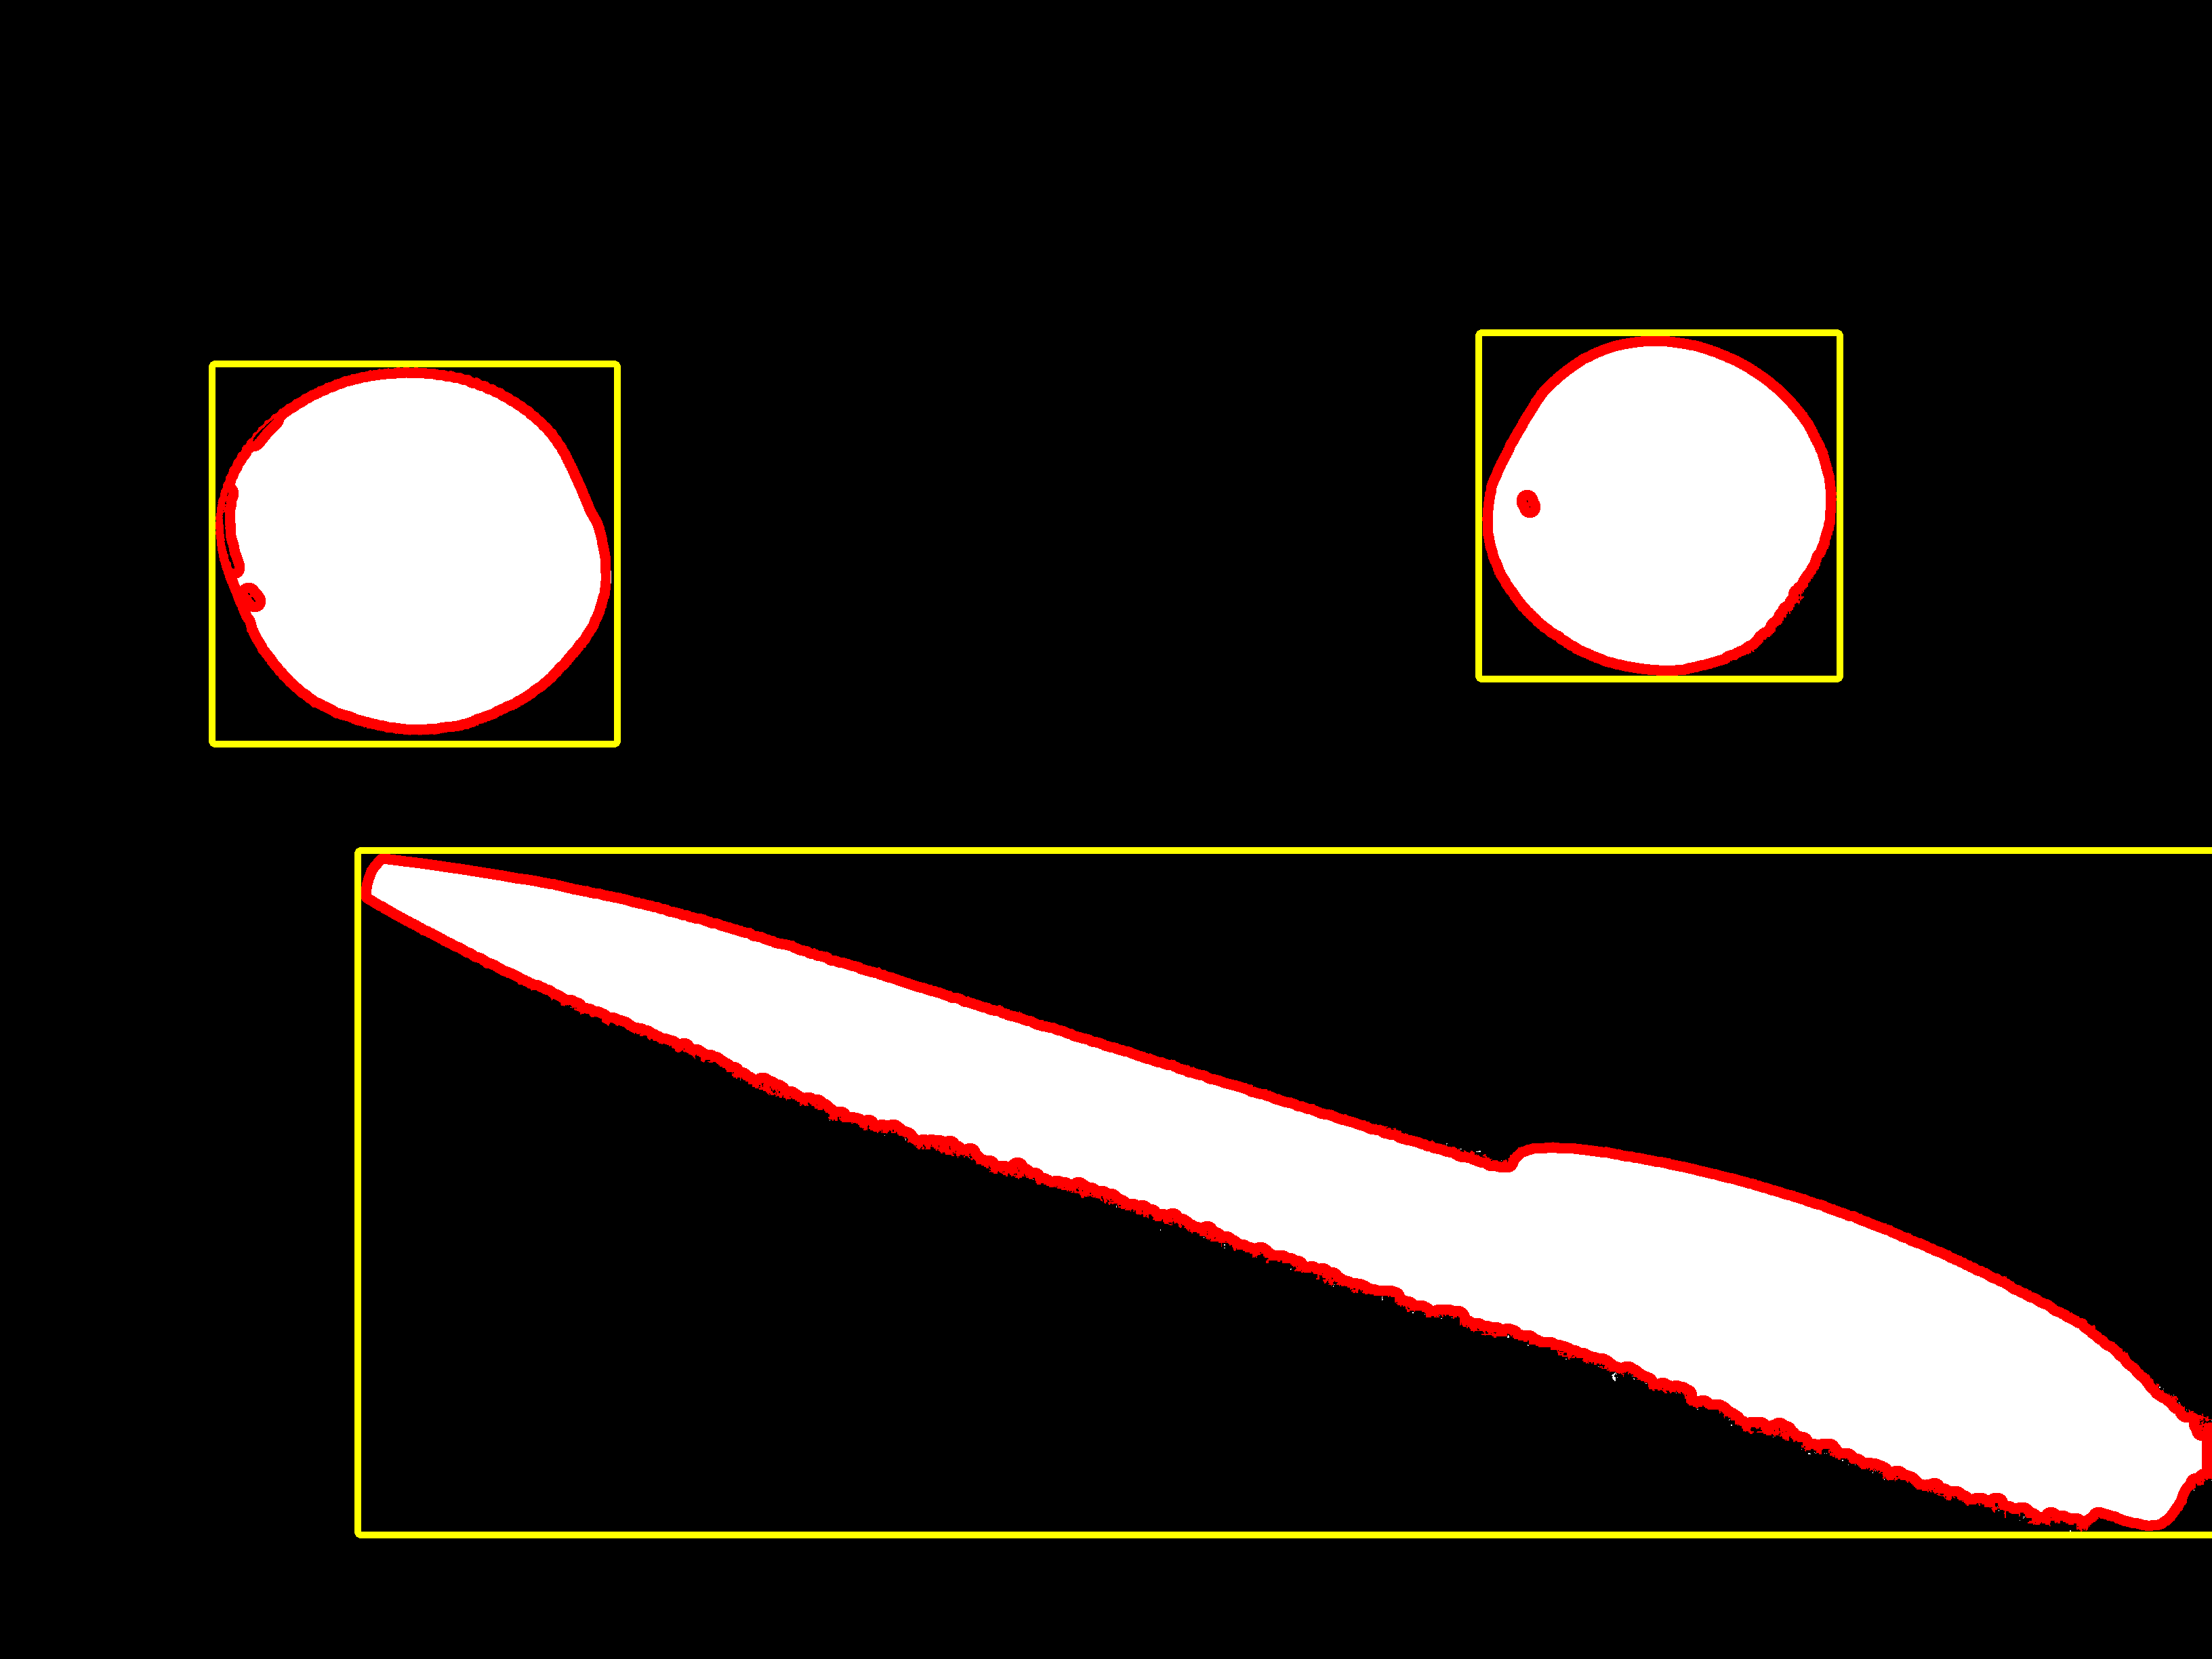
\includegraphics[width=\textwidth/2]{Bilder/Software/ColormodelsSegmentated}
\caption{Beispiel einer Segmentierung des binarisierten Sättigungskanals}
\label{fig:SegmentedColorModels}
\end{figure}

\section{Ortsbestimmung}

Die Aufgabe des Roboters ist es, Gegenstände in vordefinierte Bereiche zu befördern. Hierzu muss ihm jederzeit bekannt sein wo diese sich befinden, bzw. wo er sich relativ zu diesen aufhält, um sie anfahren zu können.

\subsection{Arten der Positionsbestimmung}

\subsubsection{Mitteilung von Beobachterkomponente}
Ist im Raum ein weiteres System vorhanden, dessen Position konstant ist und welche den Roboter stets im Blick behält (über Kameras, Ultraschall, o. Ä.), ist eine simple und doch genaue Positionsbestimmung möglich. Der Roboter muss hierbei keine Berechnungen anstellen und verlässt sich für die korrekte Positionsbestimmung ganz auf den Beobachter, von welcher jederzeit die Lage des Roboters im Raum abrufbar ist.

\subsubsection{Raumanalyse}

Hierbei werden die Kamerabilder analysiert und aus ihnen Fixpunkte/-geraden des Raumes extrahiert, mit welchen sich der Roboter bei Bewegung im Raum zu orientieren versucht. Dies setzt jedoch relativ viel Rechenzeit bei der Bildverarbeitung und Implementierungsarbeit voraus.

Auch müssen im Raum genügend Orientierungspunkte vorhanden sein. Verliert der Roboter die Orientierung, ist es nicht ohne weiteres möglich diese wiederzuerlangen.

\subsubsection{Positionsverfolgung}

Besitzt der Roboter einen möglichst exakten Sensor zur Beobachtung der eigens zurückgelegten Strecken in jede Richtung, kann er seine Position bestimmen, indem er jede Bewegung aufzeichnet und diesen Bewegungsvektor auf die letzte Position aufaddiert.

Bei Rotationssensoren in den Rädern wird die Genauigkeit diese Verfahrens durch das Spiel der Räder und der Auflösung der Sensoren beeinträchtigt.

Da bei diesem Projekt keine Beobachterkomponente vorhanden ist und die zusätzliche Auswertung der Bilder zu aufwändig wäre, wurde sich für die Variante der Positionsverfolgung entschieden. Die Auflösung der Rotationssensoren ist mit 1\degree ausreichend genau. Die automatische Geschwindigkeitsanpassung der NXT-Motoren abhängig des Untergrunds fördern zusätzlich eine exakte Ortsbestimmung über die Positionsverfolgung.

\section{Struktur der Android-App}
\subsection{Activities}
Aktivitätsdiagramm






